\documentclass[conference]{IEEEtran}
\usepackage{graphicx,booktabs,xcolor,amsmath,hyperref}
\graphicspath{{figures/}{../results/}}
\newcommand{\todo}[1]{\textcolor{red}{\textbf{[TODO: #1]}}}
\newcommand{\repo}{\url{https://github.com/Tshoki-m/Investigating-the-Effect-of-Recurrent-Processing-on-CORnet-S-Performance}}

\begin{document}
\title{Investigating the Effect of Recurrent Processing on CORnet-S Performance: A Partial Reproduction That Did Not Reproduce}
\author{\IEEEauthorblockN{\todo{Your name}}
\IEEEauthorblockA{\todo{Student number, course, University of the Witwatersrand}}}
\maketitle

\begin{abstract}
Kubilius et al.\ report that removing recurrence from CORnet-S lowers ImageNet top-1 accuracy by about 7 points (Fig.~4, row~1). I re-implemented CORnet-S and trained four variants (1/1/1, 2/2/2, 2/4/2, 4/4/4 recurrent steps in V2/V4/IT) from scratch under one shared recipe, on a reduced protocol (Tiny-ImageNet, 64$\times$64, 200 classes). The effect did \emph{not} reproduce: with one seed per configuration the non-recurrent model scored highest (+1.25 points over baseline) and 4/4/4 lowest ($-2.85$). I could not establish why, and the result should be read as no detected benefit of recurrence in a small-data, low-resolution regime, not as evidence against the original finding. Code: \repo
\end{abstract}

\section{The claim}
CORnet-S has four areas mapped to the ventral stream (V1, V2, V4, IT). V1 is feed-forward; V2, V4 and IT are recurrent: an area's output is passed back through the same weights several times, with BatchNorm kept separate per step \cite{kubilius2019}. The baseline repeats V2 twice, V4 four times and IT twice (2/4/2).

\textbf{Claim reproduced.} The abstract states that recurrence is the main predictive factor of ImageNet top-1 and Brain-Score. I test only its ImageNet part, the row ``number of recurrent steps in V2/V4/IT'' of \textbf{Fig.~4} (Sec.~4.3): relative to 2/4/2, ImageNet top-1 changes by $-7$ for no recurrence (1/1/1), $-1$ for 2/2/2, and $0$ for 4/4/4, 4/8/4 and 10/10/10 (Brain-Score: $-3$, 0, 0, 0, 0). I checked these values on the rendered figure; they are integers labelled ``\%'', and the paper does not say whether this means points or relative change.

\textbf{How the authors supported it.} They trained CORnet-S variants that each change one circuit element, kept training hyperparameters identical across variants (a caveat they state), and report the change in ImageNet top-1 and Brain-Score (V4, IT and behaviour only) against the baseline. The paper does not report seeds or error bars, nor whether variants were trained for the full 43 epochs or at which epoch they were measured. I assumed the main recipe.

\textbf{Scope.} Fig.~4 does not show recurrence to be the largest factor on ImageNet top-1: a $1\times$ bottleneck costs $-8$, comparable to $-7$ for no recurrence. Recurrence leads clearly only on Brain-Score ($-3$). I therefore test only whether recurrence matters for ImageNet top-1, not the ``main factor'' wording and not Brain-Score.

\section{My route}
I \emph{re-implemented} CORnet-S rather than running the authors' training code. \textbf{Mine:} the training and evaluation loop, data preparation, analysis and the single-command pipeline (\texttt{train.py}, \texttt{prep\_tiny\_imagenet.py}, \texttt{analyze.py}, \texttt{reproduce.py}). \textbf{Close to the authors':} \texttt{cornet\_s.py} is a re-implementation written to mirror the layout and module names of the official \texttt{dicarlolab/cornet} code, with the number of steps per area as an argument, so it is not an independent design; the official pretrained weights load into it with strict key matching. The official code was used only to validate my model. \todo{state result of the numerical output comparison (results/equivalence\_check.txt): max abs difference and pass/fail; if not run, say so}

\textbf{Tool use.} I developed the code and this report with the help of an AI assistant (Claude). \todo{state what you wrote, reviewed and ran yourself, in the form your course policy requires; keep it truthful}

\section{Protocol, and what differs from the paper}
All variants train from scratch with identical hyperparameters. Table~\ref{tab:protocol} lists every difference I know of.

\begin{table}[t]
\caption{Training protocol: paper versus this reproduction.}
\label{tab:protocol}
\centering\small
\begin{tabular}{@{}lll@{}}
\toprule
 & Paper & Here \\
\midrule
Data & ImageNet, 1000 cl. & Tiny-ImageNet, 200 cl. \\
Train/val images & 1.28M / 50k & 100k / 10k \\
Resolution & 224$\times$224 & 64$\times$64 \\
Final feature map & $7\times7$ & $2\times2$ \\
Epochs, batch & 43, 256 & 43, 256 \\
Optimizer & SGD, mom.\ 0.9 & SGD, mom.\ 0.9 \\
LR schedule & 0.1, $\div$10 / 20 ep. & same \\
Weight decay & not stated & 1e-4 (assumed) \\
Augmentation & crop, flip & RandResizedCrop (min 0.35), flip \\
Precision & not stated & mixed (AMP) \\
Reported epoch & max Brain-Score & final epoch \\
Hardware & 2 GPUs & \todo{Colab GPU model} \\
Seeds & not stated & 1 per config. \\
\bottomrule
\end{tabular}
\end{table}

Tiny-ImageNet \cite{tinyimagenet} was chosen because full ImageNet exceeds Colab's disk and its two CPU cores. I report last-epoch validation top-1 rather than selecting the best epoch on the validation set, which would bias the comparison. Total steps per variant are 3, 6, 8 and 12, with parameter counts nearly identical (about 53.0M), so variants differ in computation rather than capacity.

\section{Numbers next to the paper's}
\begin{table}[t]
\caption{Top-1 on Tiny-ImageNet validation (last epoch, one seed). $\Delta$ is relative to 2/4/2; paper $\Delta$ is ImageNet top-1 from Fig.~4; train loss is the mean loss over the last epoch (under augmentation).}
\label{tab:results}
\centering\small
\begin{tabular}{@{}lccccc c@{}}
\toprule
V2/V4/IT & Steps & Params (M) & Top-1 (\%) & $\Delta$ & Paper $\Delta$ & Train loss \\
\midrule
1/1/1 & 3 & 52.98 & 49.11 & +1.25 & $-7$ & 0.86 \\
2/2/2 & 6 & 53.00 & 48.14 & +0.28 & $-1$ & 0.73 \\
2/4/2 & 8 & 53.01 & 47.86 & 0 & 0 & 0.78 \\
4/4/4 & 12 & 53.03 & 45.01 & $-2.85$ & 0 & 1.19 \\
\bottomrule
\end{tabular}
\end{table}

\begin{figure}[t]
\centering
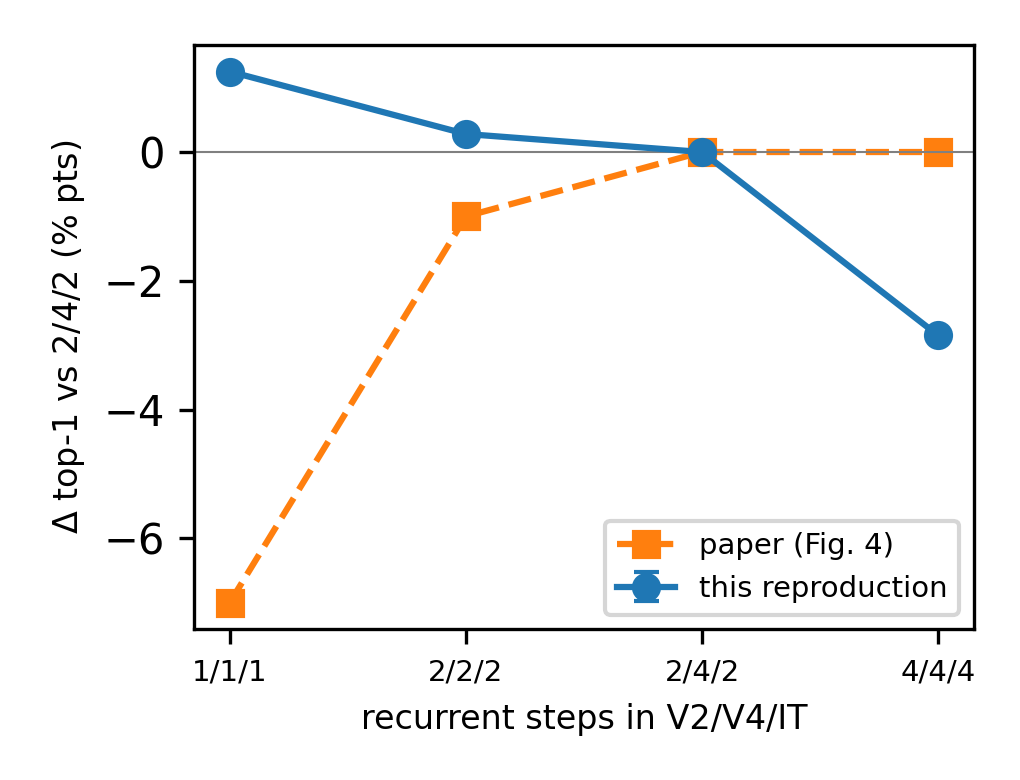
\includegraphics[width=0.85\columnwidth]{recurrence_ablation.png}
\caption{Change in top-1 relative to the 2/4/2 baseline: this reproduction (one seed, no error bars) versus the paper's Fig.~4 values.}
\label{fig:delta}
\end{figure}

The comparison is not like for like, because the dataset, resolution, class count and feature-map size all differ (Table~\ref{tab:protocol}); it asks whether the \emph{direction and rough size} of the effect survive the change of regime.

\textbf{Numbers the paper does not report.} (i) Absolute accuracies of 45.0--49.1\% per variant. (ii) Accuracy falls monotonically with total recurrent steps (3, 6, 8, 12 steps give 49.1, 48.1, 47.9, 45.0). (iii) A sampling uncertainty of about $\pm0.5$ points per accuracy, from the binomial error on 10{,}000 validation images, hence about $\pm0.7$ for a difference between two configurations. (iv) Final-epoch training loss of 0.86, 0.73, 0.78 and 1.19 for 1/1/1, 2/2/2, 2/4/2 and 4/4/4 (Table~\ref{tab:results}). (v) Best-epoch validation top-1 of 49.19, 48.49, 47.96 and 45.01, within 0.4 points of the last-epoch values, so reporting the last epoch does not change the ranking.

\textbf{How to read the differences.} A one-point gap is only about 1.4 standard errors of the difference, before training variance, which one seed cannot estimate. The 4/4/4 gap ($-2.85$) is about four standard errors and the most credible; the 1/1/1 gap (+1.25) is borderline; the 2/2/2 gap (+0.28) is indistinguishable from zero.

\section{The gap: what did not reproduce}
The central effect did not reproduce. The paper reports a large drop without recurrence; I found the opposite ordering, with the feed-forward 1/1/1 variant best and accuracy declining as steps increased. The paper's plateau above 2/4/2 did not appear either: 4/4/4 fell $2.85$ points below baseline. The honest statement is that \emph{no benefit of recurrence was detected} in this regime and that deeper unrolling probably hurt.

\textbf{What I tried.} Beyond the four runs, I analysed their saved training histories: final training loss, best-epoch accuracy and the per-epoch curves (Fig.~\ref{fig:curves}). I did not run extra seeds or any other variant. \todo{if you ran extra seeds or the no-pool variant (results\_nopool/) before submitting, describe them here and update the abstract and Table II; otherwise delete this note}

\begin{figure*}[t]
\centering
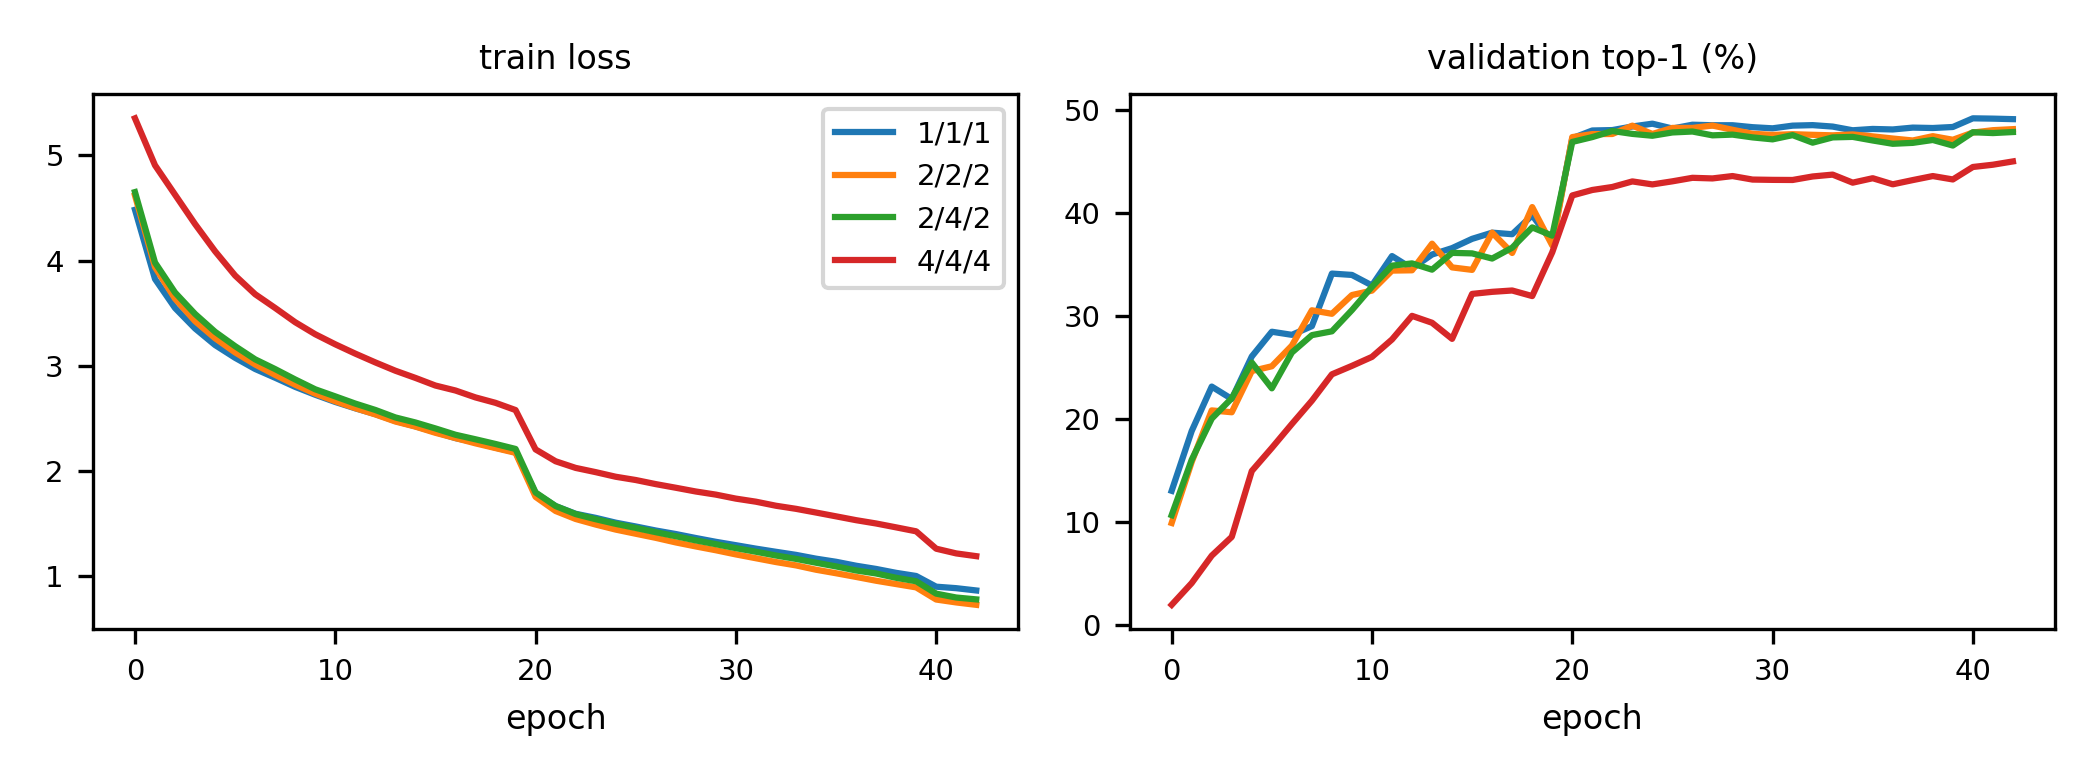
\includegraphics[width=0.85\textwidth]{training_curves.png}
\caption{Training loss (left) and validation top-1 (right) per epoch for each variant.}
\label{fig:curves}
\end{figure*}

\textbf{What the training losses show.} 4/4/4 has the \emph{highest} final training loss (1.19) as well as the lowest validation accuracy, and its best validation accuracy occurs at the last epoch, so it is not overfitting; it fits the data worse and probably had not converged under this schedule, which points to an optimization difficulty. The picture is different for the other variants: 2/2/2 and 2/4/2 reach a lower training loss than 1/1/1 (0.73 and 0.78 against 0.86) yet a lower validation accuracy, which is consistent with a larger generalization gap, but these differences are within what one seed and a 10{,}000-image validation set can resolve. The training loss is an average under augmentation, not an evaluation of the training set. \todo{add one sentence describing what Fig.~\ref{fig:curves} shows, only what is visible}

\textbf{What I cannot explain.} I have hypotheses but have not tested them:
\begin{enumerate}
\item \emph{Data regime.} The paper uses 1.28M images, 1000 classes and $224\times224$ inputs; here there are 100k images, 200 classes and a $2\times2$ final map. Extra iterations at V4 and IT may add little spatial refinement while making the unrolled network harder to optimize. Because weights are shared, each extra step lengthens the path gradients take through the same parameters, which fits the high training loss of 4/4/4, though one seed cannot establish it and it does not explain why 1/1/1 generalizes better than 2/2/2 and 2/4/2.
\item \emph{Untuned shared hyperparameters}, which the paper itself flags as a caveat; it is likely stronger with less data.
\item \emph{Recurrence confounded with depth.} With shared weights, 1/1/1 has about the same parameters as 2/4/2 but far less computation, so the paper's $-7$ mixes less recurrence with a shallower effective network \cite{liao2016}.
\item \emph{Protocol differences} (augmentation scale, mixed precision, assumed weight decay, final-epoch reporting), which could shift absolute numbers but are unlikely alone to reverse a trend.
\end{enumerate}

\section{Limitations}
(i) One seed per configuration, so differences below about one point cannot be interpreted. (ii) Reduced dataset and resolution; the result does not bear directly on the full-ImageNet claim. (iii) Brain-Score and the ``main factor'' comparison were not tested. (iv) Fig.~4's deltas are rounded integers with ambiguous units, and its training details are underspecified. (v) The original plan was to start from the authors' implementation and pretrained model, but the paper's ablation needs separately trained variants, so I trained re-implemented variants from scratch.

\section{Data ethics}
My experiments involve no data collected from people for this study and no face or person analysis. Tiny-ImageNet \cite{tinyimagenet} is a downsampled subset of ImageNet, whose images were collected from the web; some images incidentally show people, and the depicted individuals did not consent to inclusion. ImageNet is distributed for non-commercial research and educational use, which this coursework satisfies. I do not redistribute images: the repository downloads the data with a script. The original paper's Brain-Score benchmarks use monkey neural recordings; I did not use them. \todo{check the exact current terms of access for Tiny-ImageNet/ImageNet and adjust this paragraph}

\section{Reproducibility and conclusion}
The repository has a README, a pinned conda \texttt{environment.yml}, and one command, \texttt{python reproduce.py}, that downloads the data, runs the equivalence check, trains the four configurations with the protocol of Table~\ref{tab:protocol}, and regenerates every table, number and figure here. Training takes hours, so the finished run histories are committed and \texttt{python reproduce.py --skip-training} rebuilds all tables and figures from them in seconds. \todo{state the approximate wall-clock time per run}

In a reduced Tiny-ImageNet setting I found no benefit of recurrent processing for ImageNet-style top-1 accuracy in CORnet-S and a decline at 4/4/4. This does not contradict the paper's full-scale result, because the regime differs substantially, but it shows the reported benefit is not robust to a drop in data scale and resolution under a shared untuned recipe. \todo{if you ran extra seeds or the no-pool variant, update the abstract, Table~\ref{tab:results} and this paragraph to match}

\begin{thebibliography}{1}
\bibitem{kubilius2019} J.~Kubilius, M.~Schrimpf, K.~Kar, \emph{et al.}, ``Brain-like object recognition with high-performing shallow recurrent ANNs,'' in \emph{Adv.\ Neural Inf.\ Process.\ Syst.\ (NeurIPS)}, 2019.
\bibitem{tinyimagenet} Y.~Le and X.~Yang, ``Tiny ImageNet visual recognition challenge,'' CS 231N, Stanford University, 2015.
\bibitem{liao2016} Q.~Liao and T.~Poggio, ``Bridging the gaps between residual learning, recurrent neural networks and visual cortex,'' arXiv:1604.03640, 2016.
\end{thebibliography}
\end{document}
